\chapter{Directory structure}

We briefly describe the directory structure of \eWoms in terms
of subdirectories, source files, and tests. For more details,
the Doxygen documentation should be considered.
\eWoms comes in form of a DUNE module \texttt{ewoms}.
It has a similar structure as other DUNE modules like \texttt{dune-grid}.
The following subdirectories are within the module's root directory,
from now on assumed to be \texttt{/}:
\begin{itemize}
\item \texttt{CMake}: the configuration options
for building \eWoms using CMake. See the file \texttt{INSTALL.cmake} in
the root directory of the \eWoms distribution for details. Of course,
it is also possible to use the DUNE buildsystem just like for the other
DUNE modules.
\item \texttt{doc}: contains the Doxygen documentation in \texttt{doxygen},
this handbook in \texttt{handbook}, and the \eWoms logo in various formats in
\texttt{logo}. The html documentation produced by Doxygen can be accessed as usual,
namely, by opening \texttt{doc/doxygen/html/index.html} with a web browser.
\item \texttt{ewoms}: the \eWoms source files. See Section \ref{sec:ewoms} for details.
\item \texttt{test}: tests for each numerical model and the property system.
See Section \ref{sec:test} for details.
\item \texttt{tutorial}: contains the tutorials described in Chapter \ref{chp:tutorial}.
\end{itemize}


\subsection{The \texttt{ewoms} directory}\label{sec:ewoms}

The directory \texttt{ewoms} contains the \eWoms source files. It consists of the following subdirectories (see Figure \ref{fig:ewoms-structure}):

\begin{itemize}

\item \texttt{boxmodels}: The fully implicit vertex-centered finite
  volume (box) method. This directory features the following
  sub-directories
  \begin{itemize}
  \item \texttt{common}: The infrastructural code shared by all box
    models; For example it contains the file
    \texttt{boxfvelementgeometry.hh} which is used by the box scheme to
    construct the dual grid out of the primal one.
  \item \texttt{modules}: This directory features parts which can be
    re-used by multiple models, like a generic plug-in for the energy
    equation, models for determining the filter velocity, or plugins
    describing molecular diffusion.
  \item Each of the other subdirectories contains
    a physical numerical model which uses the box discretization.
  \end{itemize}

\item \texttt{common}: General stuff like the \eWoms property system
  and classes for managing time which are shared by the fully-implicit
  and the semi-implicit models.  For example it features the file
  \texttt{start.hh} which provides the default way for starting a
  simulation.

\item \texttt{io}: Additional classes that provide in-/output routines
  like writing and reading restart files (often called 'checkpoint'
  files) and for writing a series of VTK files.

\item \texttt{material}: Everything related to material parameters and
  constitutive equations. For example, the properties of a pure
  chemical substance (e.g. water) or pseudo substance (e.g. air) can
  be found in the subdirectory \texttt{components} with the base class
  \texttt{components/component.hh}. Fluid systems are located in the
  sub-folder \texttt{fluidsystems}, while capillary pressure/relative
  permeability laws are located in the sub-folder
  \texttt{fluidmatrixinteractions}. Furthermore, the classes computing
  binary coefficients like the Henry coefficient or binary diffusion
  coefficients are held by the sub-folder \texttt{binarycoefficients}.

\item \texttt{nonlinear}: This folder contains an implementation of
  the Newton-Raphson method for solving non-linear systems of
  equations.

\item \texttt{linear}: This folder features code which is required to
  parallelize the linear solvers, as well as back-ends for these
  solvers. For example it contains classes to calculate an overlap
  given the distributed matrix of the linear system, and provides
  classes which use this overlap to provide overlapping matrices,
  vectors, linear operators and scalar products.

\item \texttt{istl}: This folder contains a copy of slightly modified
  linear solvers from the ISTL \Dune module. The reason why they where
  copied is to provide linear solvers with better performance and
  stability without being held back by the \Dune developers.

\item \texttt{parallel}: Contains some helper classes useful for
  programming MPI parallel code. For example this folder contains a
  simple MPI buffer class, and various commonly used \Dune
  data-handles.
\end{itemize}

\subsection{The directory \texttt{test}}\label{sec:test}

The directory \texttt{test} contains at least one test/example for
each numerical model and for each important aspect of the common
\eWoms infrastructure. The directory \texttt{common} contains a test
for the property system.  The sub-directory \texttt{implicit}
contains test applications for the fully-implicit models (where each
test is named according to the scheme \texttt{PROBLEMNAME\_MODDEL}).
Each subdirectory contains one or more program
files \texttt{*.cc} which contain the main function for the
test. Moreover, the problem definitions can be found in the
\texttt{*problem.hh} files. Simply executing the tests should either
run the full test or give a list of required command line
arguments. After test execution, VTK output files are generated by
most tests.  For more detailed descriptions of the tests, the problem
definitions and their corresponding Doxygen documentation should be
considered.

\begin{landscape}
\begin{figure}[hbt]
  \centering
  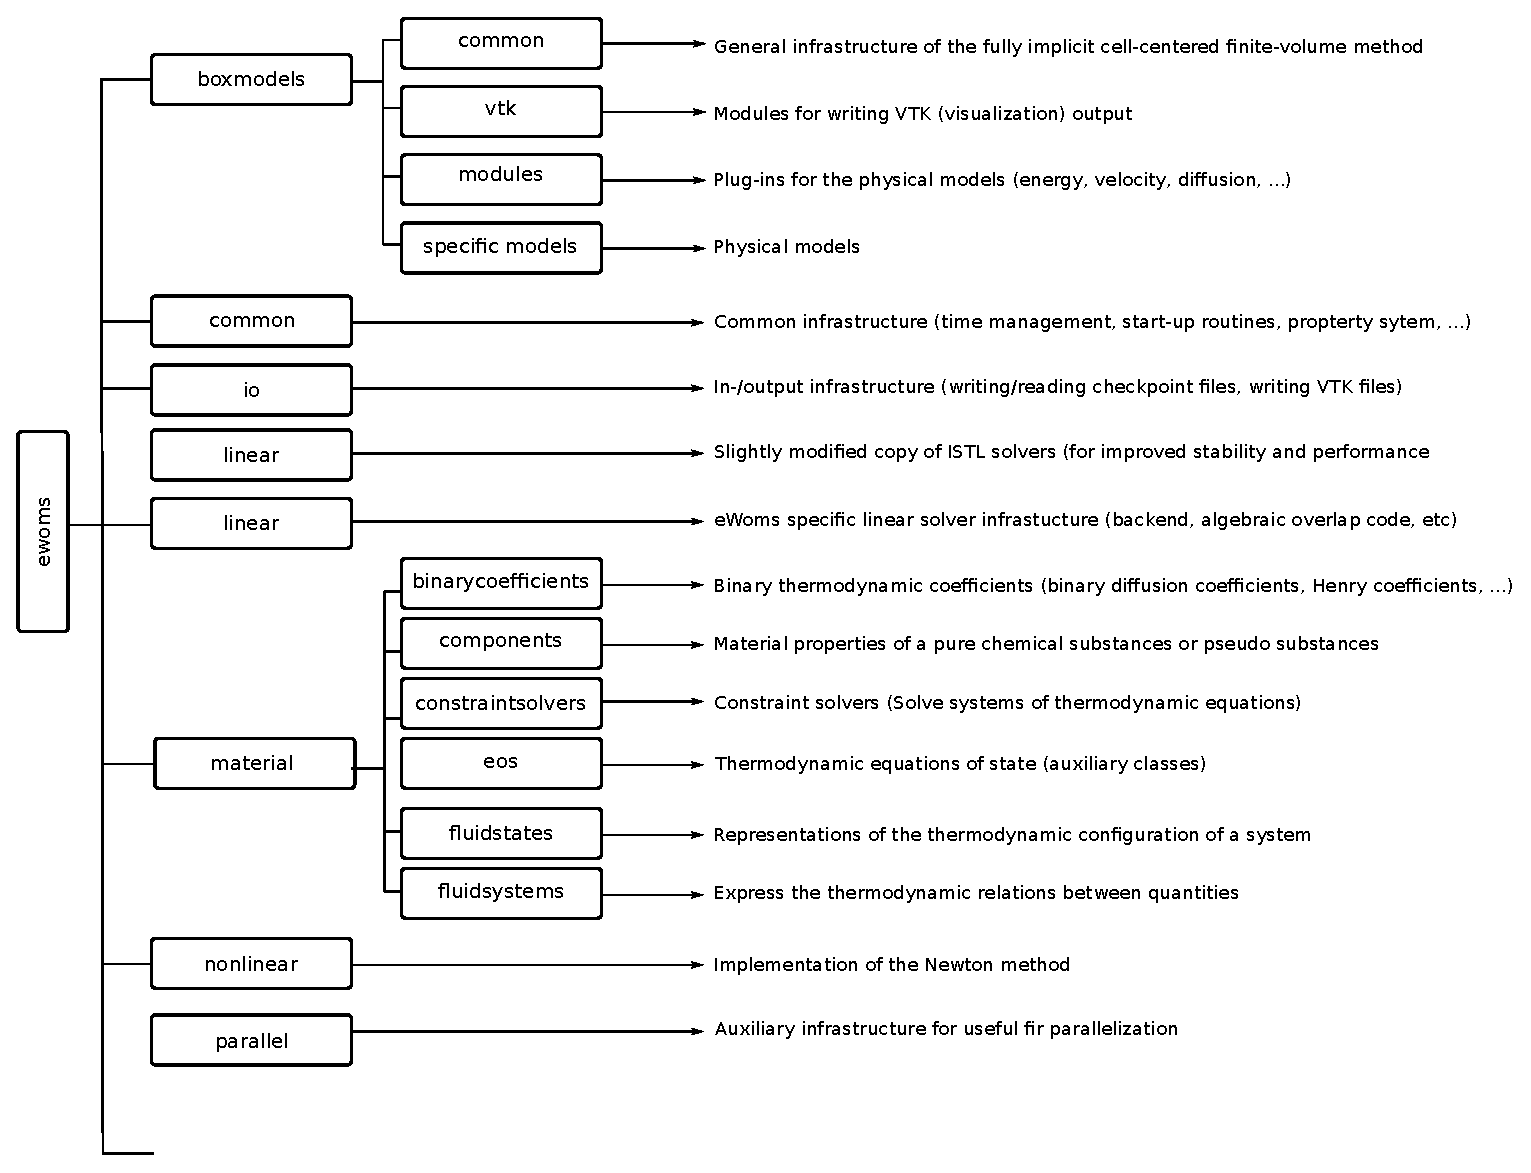
\includegraphics[width=\linewidth, keepaspectratio]{EPS/ewoms_structure.eps}
  \caption{
    \label{fig:ewoms-structure}
    Structure \texttt{ewoms} sub-directory of the \eWoms source tree.
  }
\end{figure}
\end{landscape}

%%% Local Variables:
%%% mode: latex
%%% TeX-master: "ewoms-handbook"
%%% End:
